% Created by tikzDevice version 0.10.1 on 2016-07-30 21:53:57
% !TEX encoding = UTF-8 Unicode
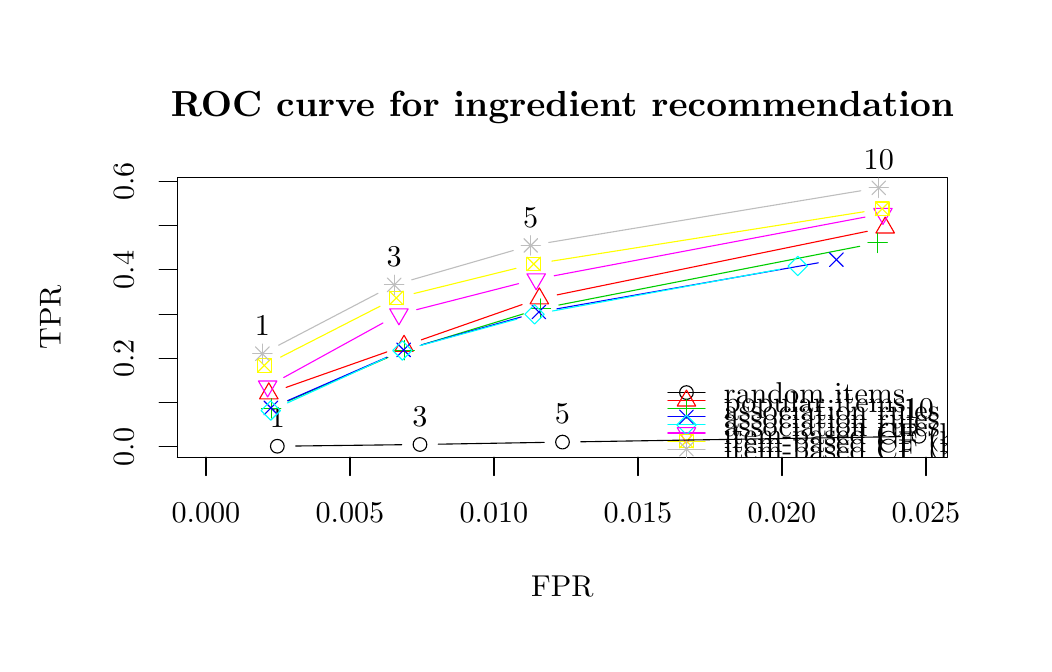
\begin{tikzpicture}[x=1pt,y=1pt]
\definecolor{fillColor}{RGB}{255,255,255}
\path[use as bounding box,fill=fillColor,fill opacity=0.00] (0,0) rectangle (360.07,222.54);
\begin{scope}
\path[clip] (  0.00,  0.00) rectangle (360.07,222.54);
\definecolor{drawColor}{RGB}{0,0,0}

\path[draw=drawColor,line width= 0.4pt,line join=round,line cap=round] ( 64.42, 67.32) -- (324.60, 67.32);

\path[draw=drawColor,line width= 0.4pt,line join=round,line cap=round] ( 64.42, 67.32) -- ( 64.42, 60.72);

\path[draw=drawColor,line width= 0.4pt,line join=round,line cap=round] (116.46, 67.32) -- (116.46, 60.72);

\path[draw=drawColor,line width= 0.4pt,line join=round,line cap=round] (168.49, 67.32) -- (168.49, 60.72);

\path[draw=drawColor,line width= 0.4pt,line join=round,line cap=round] (220.53, 67.32) -- (220.53, 60.72);

\path[draw=drawColor,line width= 0.4pt,line join=round,line cap=round] (272.56, 67.32) -- (272.56, 60.72);

\path[draw=drawColor,line width= 0.4pt,line join=round,line cap=round] (324.60, 67.32) -- (324.60, 60.72);

\node[text=drawColor,anchor=base,inner sep=0pt, outer sep=0pt, scale=  1.09] at ( 64.42, 43.56) {0.000};

\node[text=drawColor,anchor=base,inner sep=0pt, outer sep=0pt, scale=  1.09] at (116.46, 43.56) {0.005};

\node[text=drawColor,anchor=base,inner sep=0pt, outer sep=0pt, scale=  1.09] at (168.49, 43.56) {0.010};

\node[text=drawColor,anchor=base,inner sep=0pt, outer sep=0pt, scale=  1.09] at (220.53, 43.56) {0.015};

\node[text=drawColor,anchor=base,inner sep=0pt, outer sep=0pt, scale=  1.09] at (272.56, 43.56) {0.020};

\node[text=drawColor,anchor=base,inner sep=0pt, outer sep=0pt, scale=  1.09] at (324.60, 43.56) {0.025};

\path[draw=drawColor,line width= 0.4pt,line join=round,line cap=round] ( 54.12, 71.06) -- ( 54.12,166.98);

\path[draw=drawColor,line width= 0.4pt,line join=round,line cap=round] ( 54.12, 71.06) -- ( 47.52, 71.06);

\path[draw=drawColor,line width= 0.4pt,line join=round,line cap=round] ( 54.12, 87.05) -- ( 47.52, 87.05);

\path[draw=drawColor,line width= 0.4pt,line join=round,line cap=round] ( 54.12,103.03) -- ( 47.52,103.03);

\path[draw=drawColor,line width= 0.4pt,line join=round,line cap=round] ( 54.12,119.02) -- ( 47.52,119.02);

\path[draw=drawColor,line width= 0.4pt,line join=round,line cap=round] ( 54.12,135.01) -- ( 47.52,135.01);

\path[draw=drawColor,line width= 0.4pt,line join=round,line cap=round] ( 54.12,150.99) -- ( 47.52,150.99);

\path[draw=drawColor,line width= 0.4pt,line join=round,line cap=round] ( 54.12,166.98) -- ( 47.52,166.98);

\node[text=drawColor,rotate= 90.00,anchor=base,inner sep=0pt, outer sep=0pt, scale=  1.09] at ( 38.28, 71.06) {0.0};

\node[text=drawColor,rotate= 90.00,anchor=base,inner sep=0pt, outer sep=0pt, scale=  1.09] at ( 38.28,103.03) {0.2};

\node[text=drawColor,rotate= 90.00,anchor=base,inner sep=0pt, outer sep=0pt, scale=  1.09] at ( 38.28,135.01) {0.4};

\node[text=drawColor,rotate= 90.00,anchor=base,inner sep=0pt, outer sep=0pt, scale=  1.09] at ( 38.28,166.98) {0.6};

\path[draw=drawColor,line width= 0.4pt,line join=round,line cap=round] ( 54.12, 67.32) --
	(332.35, 67.32) --
	(332.35,168.42) --
	( 54.12,168.42) --
	( 54.12, 67.32);
\end{scope}
\begin{scope}
\path[clip] (  0.00,  0.00) rectangle (360.07,222.54);
\definecolor{drawColor}{RGB}{0,0,0}

\node[text=drawColor,anchor=base,inner sep=0pt, outer sep=0pt, scale=  1.09] at (193.24, 17.16) {FPR};

\node[text=drawColor,rotate= 90.00,anchor=base,inner sep=0pt, outer sep=0pt, scale=  1.09] at ( 11.88,117.87) {TPR};
\end{scope}
\begin{scope}
\path[clip] ( 54.12, 67.32) rectangle (332.35,168.42);
\definecolor{drawColor}{RGB}{0,0,0}

\path[draw=drawColor,line width= 0.4pt,line join=round,line cap=round] (231.31, 90.68) -- (244.80, 90.68);
\definecolor{drawColor}{RGB}{255,0,0}

\path[draw=drawColor,line width= 0.4pt,line join=round,line cap=round] (231.31, 87.76) -- (244.80, 87.76);
\definecolor{drawColor}{RGB}{0,205,0}

\path[draw=drawColor,line width= 0.4pt,line join=round,line cap=round] (231.31, 84.84) -- (244.80, 84.84);
\definecolor{drawColor}{RGB}{0,0,255}

\path[draw=drawColor,line width= 0.4pt,line join=round,line cap=round] (231.31, 81.92) -- (244.80, 81.92);
\definecolor{drawColor}{RGB}{0,255,255}

\path[draw=drawColor,line width= 0.4pt,line join=round,line cap=round] (231.31, 79.00) -- (244.80, 79.00);
\definecolor{drawColor}{RGB}{255,0,255}

\path[draw=drawColor,line width= 0.4pt,line join=round,line cap=round] (231.31, 76.08) -- (244.80, 76.08);
\definecolor{drawColor}{RGB}{255,255,0}

\path[draw=drawColor,line width= 0.4pt,line join=round,line cap=round] (231.31, 73.16) -- (244.80, 73.16);
\definecolor{drawColor}{RGB}{190,190,190}

\path[draw=drawColor,line width= 0.4pt,line join=round,line cap=round] (231.31, 70.24) -- (244.80, 70.24);
\definecolor{drawColor}{RGB}{0,0,0}

\path[draw=drawColor,line width= 0.4pt,line join=round,line cap=round] (238.05, 90.68) circle (  2.47);
\definecolor{drawColor}{RGB}{255,0,0}

\path[draw=drawColor,line width= 0.4pt,line join=round,line cap=round] (238.05, 91.61) --
	(241.39, 85.84) --
	(234.72, 85.84) --
	(238.05, 91.61);
\definecolor{drawColor}{RGB}{0,205,0}

\path[draw=drawColor,line width= 0.4pt,line join=round,line cap=round] (234.55, 84.84) -- (241.55, 84.84);

\path[draw=drawColor,line width= 0.4pt,line join=round,line cap=round] (238.05, 81.34) -- (238.05, 88.34);
\definecolor{drawColor}{RGB}{0,0,255}

\path[draw=drawColor,line width= 0.4pt,line join=round,line cap=round] (235.58, 79.45) -- (240.53, 84.40);

\path[draw=drawColor,line width= 0.4pt,line join=round,line cap=round] (235.58, 84.40) -- (240.53, 79.45);
\definecolor{drawColor}{RGB}{0,255,255}

\path[draw=drawColor,line width= 0.4pt,line join=round,line cap=round] (234.55, 79.00) --
	(238.05, 82.50) --
	(241.55, 79.00) --
	(238.05, 75.50) --
	(234.55, 79.00);
\definecolor{drawColor}{RGB}{255,0,255}

\path[draw=drawColor,line width= 0.4pt,line join=round,line cap=round] (238.05, 72.23) --
	(241.39, 78.01) --
	(234.72, 78.01) --
	(238.05, 72.23);
\definecolor{drawColor}{RGB}{255,255,0}

\path[draw=drawColor,line width= 0.4pt,line join=round,line cap=round] (235.58, 70.69) rectangle (240.53, 75.64);

\path[draw=drawColor,line width= 0.4pt,line join=round,line cap=round] (235.58, 70.69) -- (240.53, 75.64);

\path[draw=drawColor,line width= 0.4pt,line join=round,line cap=round] (235.58, 75.64) -- (240.53, 70.69);
\definecolor{drawColor}{RGB}{190,190,190}

\path[draw=drawColor,line width= 0.4pt,line join=round,line cap=round] (235.58, 67.77) -- (240.53, 72.72);

\path[draw=drawColor,line width= 0.4pt,line join=round,line cap=round] (235.58, 72.72) -- (240.53, 67.77);

\path[draw=drawColor,line width= 0.4pt,line join=round,line cap=round] (234.55, 70.24) -- (241.55, 70.24);

\path[draw=drawColor,line width= 0.4pt,line join=round,line cap=round] (238.05, 66.74) -- (238.05, 73.74);
\definecolor{drawColor}{RGB}{0,0,0}

\node[text=drawColor,anchor=base west,inner sep=0pt, outer sep=0pt, scale=  1.09] at (251.54, 86.57) {random items};

\node[text=drawColor,anchor=base west,inner sep=0pt, outer sep=0pt, scale=  1.09] at (251.54, 83.65) {popular items};

\node[text=drawColor,anchor=base west,inner sep=0pt, outer sep=0pt, scale=  1.09] at (251.54, 80.73) {association rules (0.01)};

\node[text=drawColor,anchor=base west,inner sep=0pt, outer sep=0pt, scale=  1.09] at (251.54, 77.81) {association rules (0.05)};

\node[text=drawColor,anchor=base west,inner sep=0pt, outer sep=0pt, scale=  1.09] at (251.54, 74.89) {association rules (0.1)};

\node[text=drawColor,anchor=base west,inner sep=0pt, outer sep=0pt, scale=  1.09] at (251.54, 71.97) {item-based CF (k=20)};

\node[text=drawColor,anchor=base west,inner sep=0pt, outer sep=0pt, scale=  1.09] at (251.54, 69.05) {item-based CF (k=40)};

\node[text=drawColor,anchor=base west,inner sep=0pt, outer sep=0pt, scale=  1.09] at (251.54, 66.13) {item-based CF (k=200)};

\path[draw=drawColor,line width= 0.4pt,line join=round,line cap=round] ( 96.81, 71.37) -- (135.16, 71.84);

\path[draw=drawColor,line width= 0.4pt,line join=round,line cap=round] (148.36, 72.03) -- (186.67, 72.68);

\path[draw=drawColor,line width= 0.4pt,line join=round,line cap=round] (199.86, 72.90) -- (315.45, 74.77);

\path[draw=drawColor,line width= 0.4pt,line join=round,line cap=round] ( 90.21, 71.29) circle (  2.47);

\path[draw=drawColor,line width= 0.4pt,line join=round,line cap=round] (141.76, 71.92) circle (  2.47);

\path[draw=drawColor,line width= 0.4pt,line join=round,line cap=round] (193.26, 72.79) circle (  2.47);

\path[draw=drawColor,line width= 0.4pt,line join=round,line cap=round] (322.05, 74.88) circle (  2.47);
\end{scope}
\begin{scope}
\path[clip] (  0.00,  0.00) rectangle (360.07,222.54);
\definecolor{drawColor}{RGB}{0,0,0}

\node[text=drawColor,anchor=base,inner sep=0pt, outer sep=0pt, scale=  1.09] at ( 90.21, 77.89) {1};

\node[text=drawColor,anchor=base,inner sep=0pt, outer sep=0pt, scale=  1.09] at (141.76, 78.52) {3};

\node[text=drawColor,anchor=base,inner sep=0pt, outer sep=0pt, scale=  1.09] at (193.26, 79.39) {5};

\node[text=drawColor,anchor=base,inner sep=0pt, outer sep=0pt, scale=  1.09] at (322.05, 81.48) {10};
\end{scope}
\begin{scope}
\path[clip] ( 54.12, 67.32) rectangle (332.35,168.42);
\definecolor{drawColor}{RGB}{255,0,0}

\path[draw=drawColor,line width= 0.4pt,line join=round,line cap=round] ( 93.36, 92.54) -- (129.78,105.36);

\path[draw=drawColor,line width= 0.4pt,line join=round,line cap=round] (142.23,109.73) -- (178.66,122.48);

\path[draw=drawColor,line width= 0.4pt,line join=round,line cap=round] (191.35,125.99) -- (303.40,148.96);

\path[draw=drawColor,line width= 0.4pt,line join=round,line cap=round] ( 87.13, 94.20) --
	( 90.47, 88.43) --
	( 83.80, 88.43) --
	( 87.13, 94.20);

\path[draw=drawColor,line width= 0.4pt,line join=round,line cap=round] (136.00,111.40) --
	(139.33,105.63) --
	(132.67,105.63) --
	(136.00,111.40);

\path[draw=drawColor,line width= 0.4pt,line join=round,line cap=round] (184.89,128.51) --
	(188.22,122.74) --
	(181.55,122.74) --
	(184.89,128.51);

\path[draw=drawColor,line width= 0.4pt,line join=round,line cap=round] (309.87,154.13) --
	(313.20,148.36) --
	(306.53,148.36) --
	(309.87,154.13);
\definecolor{drawColor}{RGB}{0,205,0}

\path[draw=drawColor,line width= 0.4pt,line join=round,line cap=round] ( 94.05, 87.60) -- (130.19,103.38);

\path[draw=drawColor,line width= 0.4pt,line join=round,line cap=round] (142.55,107.95) -- (179.13,119.12);

\path[draw=drawColor,line width= 0.4pt,line join=round,line cap=round] (191.93,122.31) -- (300.66,143.54);

\path[draw=drawColor,line width= 0.4pt,line join=round,line cap=round] ( 84.50, 84.96) -- ( 91.50, 84.96);

\path[draw=drawColor,line width= 0.4pt,line join=round,line cap=round] ( 88.00, 81.46) -- ( 88.00, 88.46);

\path[draw=drawColor,line width= 0.4pt,line join=round,line cap=round] (132.74,106.03) -- (139.74,106.03);

\path[draw=drawColor,line width= 0.4pt,line join=round,line cap=round] (136.24,102.53) -- (136.24,109.53);

\path[draw=drawColor,line width= 0.4pt,line join=round,line cap=round] (181.95,121.05) -- (188.95,121.05);

\path[draw=drawColor,line width= 0.4pt,line join=round,line cap=round] (185.45,117.55) -- (185.45,124.55);

\path[draw=drawColor,line width= 0.4pt,line join=round,line cap=round] (303.64,144.80) -- (310.64,144.80);

\path[draw=drawColor,line width= 0.4pt,line join=round,line cap=round] (307.14,141.30) -- (307.14,148.30);
\definecolor{drawColor}{RGB}{0,0,255}

\path[draw=drawColor,line width= 0.4pt,line join=round,line cap=round] ( 93.96, 87.77) -- (129.82,103.45);

\path[draw=drawColor,line width= 0.4pt,line join=round,line cap=round] (142.22,107.88) -- (178.35,118.01);

\path[draw=drawColor,line width= 0.4pt,line join=round,line cap=round] (191.20,120.93) -- (285.72,137.57);

\path[draw=drawColor,line width= 0.4pt,line join=round,line cap=round] ( 85.44, 82.65) -- ( 90.39, 87.60);

\path[draw=drawColor,line width= 0.4pt,line join=round,line cap=round] ( 85.44, 87.60) -- ( 90.39, 82.65);

\path[draw=drawColor,line width= 0.4pt,line join=round,line cap=round] (133.39,103.62) -- (138.34,108.57);

\path[draw=drawColor,line width= 0.4pt,line join=round,line cap=round] (133.39,108.57) -- (138.34,103.62);

\path[draw=drawColor,line width= 0.4pt,line join=round,line cap=round] (182.23,117.32) -- (187.18,122.27);

\path[draw=drawColor,line width= 0.4pt,line join=round,line cap=round] (182.23,122.27) -- (187.18,117.32);

\path[draw=drawColor,line width= 0.4pt,line join=round,line cap=round] (289.75,136.24) -- (294.70,141.19);

\path[draw=drawColor,line width= 0.4pt,line join=round,line cap=round] (289.75,141.19) -- (294.70,136.24);
\definecolor{drawColor}{RGB}{0,255,255}

\path[draw=drawColor,line width= 0.4pt,line join=round,line cap=round] ( 93.84, 86.92) -- (129.39,103.17);

\path[draw=drawColor,line width= 0.4pt,line join=round,line cap=round] (141.76,107.65) -- (176.80,117.22);

\path[draw=drawColor,line width= 0.4pt,line join=round,line cap=round] (189.65,120.15) -- (271.79,135.24);

\path[draw=drawColor,line width= 0.4pt,line join=round,line cap=round] ( 84.34, 84.18) --
	( 87.84, 87.68) --
	( 91.34, 84.18) --
	( 87.84, 80.68) --
	( 84.34, 84.18);

\path[draw=drawColor,line width= 0.4pt,line join=round,line cap=round] (131.90,105.91) --
	(135.40,109.41) --
	(138.90,105.91) --
	(135.40,102.41) --
	(131.90,105.91);

\path[draw=drawColor,line width= 0.4pt,line join=round,line cap=round] (179.66,118.96) --
	(183.16,122.46) --
	(186.66,118.96) --
	(183.16,115.46) --
	(179.66,118.96);

\path[draw=drawColor,line width= 0.4pt,line join=round,line cap=round] (274.78,136.43) --
	(278.28,139.93) --
	(281.78,136.43) --
	(278.28,132.93) --
	(274.78,136.43);
\definecolor{drawColor}{RGB}{255,0,255}

\path[draw=drawColor,line width= 0.4pt,line join=round,line cap=round] ( 92.50, 96.11) -- (128.37,115.83);

\path[draw=drawColor,line width= 0.4pt,line join=round,line cap=round] (140.55,120.64) -- (177.36,130.04);

\path[draw=drawColor,line width= 0.4pt,line join=round,line cap=round] (190.24,132.89) -- (302.57,154.09);

\path[draw=drawColor,line width= 0.4pt,line join=round,line cap=round] ( 86.72, 89.09) --
	( 90.05, 94.86) --
	( 83.38, 94.86) --
	( 86.72, 89.09);

\path[draw=drawColor,line width= 0.4pt,line join=round,line cap=round] (134.15,115.16) --
	(137.48,120.93) --
	(130.82,120.93) --
	(134.15,115.16);

\path[draw=drawColor,line width= 0.4pt,line join=round,line cap=round] (183.75,127.82) --
	(187.09,133.59) --
	(180.42,133.59) --
	(183.75,127.82);

\path[draw=drawColor,line width= 0.4pt,line join=round,line cap=round] (309.05,151.46) --
	(312.39,157.24) --
	(305.72,157.24) --
	(309.05,151.46);
\definecolor{drawColor}{RGB}{255,255,0}

\path[draw=drawColor,line width= 0.4pt,line join=round,line cap=round] ( 91.37,103.49) -- (127.33,121.88);

\path[draw=drawColor,line width= 0.4pt,line join=round,line cap=round] (139.61,126.47) -- (176.46,135.57);

\path[draw=drawColor,line width= 0.4pt,line join=round,line cap=round] (189.39,138.18) -- (302.25,156.03);

\path[draw=drawColor,line width= 0.4pt,line join=round,line cap=round] ( 83.02, 98.00) rectangle ( 87.97,102.95);

\path[draw=drawColor,line width= 0.4pt,line join=round,line cap=round] ( 83.02, 98.00) -- ( 87.97,102.95);

\path[draw=drawColor,line width= 0.4pt,line join=round,line cap=round] ( 83.02,102.95) -- ( 87.97, 98.00);

\path[draw=drawColor,line width= 0.4pt,line join=round,line cap=round] (130.73,122.41) rectangle (135.68,127.36);

\path[draw=drawColor,line width= 0.4pt,line join=round,line cap=round] (130.73,122.41) -- (135.68,127.36);

\path[draw=drawColor,line width= 0.4pt,line join=round,line cap=round] (130.73,127.36) -- (135.68,122.41);

\path[draw=drawColor,line width= 0.4pt,line join=round,line cap=round] (180.39,134.67) rectangle (185.34,139.62);

\path[draw=drawColor,line width= 0.4pt,line join=round,line cap=round] (180.39,134.67) -- (185.34,139.62);

\path[draw=drawColor,line width= 0.4pt,line join=round,line cap=round] (180.39,139.62) -- (185.34,134.67);

\path[draw=drawColor,line width= 0.4pt,line join=round,line cap=round] (306.29,154.59) rectangle (311.24,159.54);

\path[draw=drawColor,line width= 0.4pt,line join=round,line cap=round] (306.29,154.59) -- (311.24,159.54);

\path[draw=drawColor,line width= 0.4pt,line join=round,line cap=round] (306.29,159.54) -- (311.24,154.59);
\definecolor{drawColor}{RGB}{190,190,190}

\path[draw=drawColor,line width= 0.4pt,line join=round,line cap=round] ( 90.66,107.78) -- (126.59,126.55);

\path[draw=drawColor,line width= 0.4pt,line join=round,line cap=round] (138.78,131.43) -- (175.45,142.01);

\path[draw=drawColor,line width= 0.4pt,line join=round,line cap=round] (188.30,144.92) -- (301.03,163.60);

\path[draw=drawColor,line width= 0.4pt,line join=round,line cap=round] ( 82.34,102.25) -- ( 87.29,107.20);

\path[draw=drawColor,line width= 0.4pt,line join=round,line cap=round] ( 82.34,107.20) -- ( 87.29,102.25);

\path[draw=drawColor,line width= 0.4pt,line join=round,line cap=round] ( 81.31,104.72) -- ( 88.31,104.72);

\path[draw=drawColor,line width= 0.4pt,line join=round,line cap=round] ( 84.81,101.22) -- ( 84.81,108.22);

\path[draw=drawColor,line width= 0.4pt,line join=round,line cap=round] (129.96,127.13) -- (134.91,132.08);

\path[draw=drawColor,line width= 0.4pt,line join=round,line cap=round] (129.96,132.08) -- (134.91,127.13);

\path[draw=drawColor,line width= 0.4pt,line join=round,line cap=round] (128.94,129.60) -- (135.94,129.60);

\path[draw=drawColor,line width= 0.4pt,line join=round,line cap=round] (132.44,126.10) -- (132.44,133.10);

\path[draw=drawColor,line width= 0.4pt,line join=round,line cap=round] (179.31,141.36) -- (184.26,146.31);

\path[draw=drawColor,line width= 0.4pt,line join=round,line cap=round] (179.31,146.31) -- (184.26,141.36);

\path[draw=drawColor,line width= 0.4pt,line join=round,line cap=round] (178.29,143.84) -- (185.29,143.84);

\path[draw=drawColor,line width= 0.4pt,line join=round,line cap=round] (181.79,140.34) -- (181.79,147.34);

\path[draw=drawColor,line width= 0.4pt,line join=round,line cap=round] (305.06,162.20) -- (310.01,167.15);

\path[draw=drawColor,line width= 0.4pt,line join=round,line cap=round] (305.06,167.15) -- (310.01,162.20);

\path[draw=drawColor,line width= 0.4pt,line join=round,line cap=round] (304.04,164.68) -- (311.04,164.68);

\path[draw=drawColor,line width= 0.4pt,line join=round,line cap=round] (307.54,161.18) -- (307.54,168.18);
\end{scope}
\begin{scope}
\path[clip] (  0.00,  0.00) rectangle (360.07,222.54);
\definecolor{drawColor}{RGB}{0,0,0}

\node[text=drawColor,anchor=base,inner sep=0pt, outer sep=0pt, scale=  1.09] at ( 84.81,111.32) {1};

\node[text=drawColor,anchor=base,inner sep=0pt, outer sep=0pt, scale=  1.09] at (132.44,136.20) {3};

\node[text=drawColor,anchor=base,inner sep=0pt, outer sep=0pt, scale=  1.09] at (181.79,150.44) {5};

\node[text=drawColor,anchor=base,inner sep=0pt, outer sep=0pt, scale=  1.09] at (307.54,171.28) {10};

\node[text=drawColor,anchor=base,inner sep=0pt, outer sep=0pt, scale=  1.31] at (193.24,190.53) {\bfseries ROC curve for ingredient recommendation};
\end{scope}
\end{tikzpicture}
